\documentclass[a4paper,12pt]{article}
\usepackage[left=2cm,right=2cm,top=2cm,bottom=2cm]{geometry} % Do ustawień marginesów
\usepackage{multicol} % Dla podziału na kolumny
\usepackage{ragged2e} % Dla justowania tekstu
\usepackage{graphicx} % Required for inserting images
\usepackage{float}
\usepackage{caption}
\usepackage{amsmath} % Math formulas
\usepackage{amssymb} % Symbols
\usepackage[svgnames]{xcolor}
\usepackage[colorlinks=true, urlcolor=blue, linkcolor=black, citecolor=orange]{hyperref} % Hyperlinks
\usepackage{polski} % Polish language
\usepackage[utf8]{inputenc} % Text encoding
\usepackage{enumitem} % Pakiet do elastycznego sterowania listami
\usepackage{indentfirst}
\usepackage{array}
\usepackage{booktabs}
\usepackage{multirow}

\begin{document}

% Górna część strony
\noindent
\begin{minipage}{0.5\textwidth}
    \raggedright
    \textbf{Piotr Durniat} \\
    I rok, Fizyka \\
    Wtorek, 8:00-10:15 \\
    \vspace{0.5cm}
    \vspace{0.5cm}
\end{minipage}%
\begin{minipage}{0.5\textwidth}
    \raggedleft
    Data wykonania pomiarów: \\
    4 marca 2025 r. \\
    \vspace{0.5cm} % Dodatkowa linia przerwy
    Prowadząca: \\
    dr Iwona Mróz
\end{minipage}

% Tytuł ćwiczenia
\vspace{2cm} % Odstęp
\begin{center}
    \LARGE \textbf{Ćwiczenie nr 9} \\[0.5cm]
    \Large \textbf{Wyznaczanie modułu Younga metodą jednostronnego rozciągania}
\end{center}

% Reszta treści
\vspace{1cm} % Kolejny odstęp
\noindent

\tableofcontents
\newpage

\section{Wstęp teoretyczny}


% • własności sprężyste ciał stałych, rodzaje deformacji ciał stałych, odkształcenie bezwzględne i względne;
Gdy na ciało stałe działa siła zewnętrzna, jego struktura ulega odkształceniu - zmianie kształtu lub rozmiaru. W przypadku niewielkich sił ciało może powrócić do swojej pierwotnej postaci po ustaniu działania siły - takie odkształcenie nazywane jest odkształceniem sprężystym. W przypadku jednak, gdy wartość siły przekroczy granicę sprężystości, odkształcenie stanie się trwałe - takie odkształcenie nazywane jest odkształceniem plastycznym.

% prawo Hooke’a i zakres jego stosowalności, współczynniki charakteryzujące własności sprężyste ciał oraz zależności między nimi;

W zakresie odkształceń sprężystych zachodzi prawo Hooke'a, które stwierdza, że ciśnienie ($p$) wewnątrz ciała jest proporcjonalne do odkształcenia względnego ($\alpha$):

\begin{equation} \label{eq:prawo_hookea}
    p = k\alpha
\end{equation}

gdzie:
\begin{itemize}
    \setlength{\itemsep}{0em}
    \item $p$ - ciśnienie,
    \item $k$ - współczynnik proporcjonalności zwany modułem sprężystości,
    \item $\alpha$ - odkształcenie względne.
\end{itemize}

Prawo Hooke’a obowiązuje tylko w zakresie sprężystości. Po przekroczeniu granicznego naprężenia, materiał przechodzi w zakres plastyczny, a zależność ta przestaje być liniowa.



% TODO: współczynniki charakteryzujące własności sprężyste ciał oraz zależności między nimi?

% • definicja i wymiar modułu Younga;

Moduł Younga ($E$) jest stałą sprężystości materiału, która określa moduł sprężystości dla deformacji wydłużania. W przypadku odkształcenia wydłużającego, odkształcenie względne jest określone jako stosunek wydłużenia bezwzględnego $\Delta{l}$ do początkowej długości ciała $l$:
$$
    \alpha = \frac{\Delta l}{l}
$$
Podstawiając te zależności do prawa Hooke’a (\ref{eq:prawo_hookea}), moduł Younga można zapisać w postaci:

\begin{equation} \label{eq:modul_younga}
    E = \frac{Fl}{q \Delta l}
\end{equation}

gdzie:
\begin{itemize}
    \setlength{\itemsep}{0em}
    \item $F$ – siła rozciągająca,
    \item $l$ – początkowa długość próbki,
    \item $q$ – pole przekroju poprzecznego materiału,
    \item $\Delta l$ – wydłużenie próbki pod wpływem siły.
\end{itemize}
Moduł Younga ma wymiar ciśnienia i jest wyrażany w paskalach $[\text{Pa}]$.
% • sposób wyznaczania modułu Younga metodą jednostronnego rozciągania i inne metody wyznaczania modułu Younga
Do wyznaczenia wartości modułu Younga można skorzystać z metody jednostronnego rozciągania, wykorzystując zależność podaną w równaniu~(\ref{eq:modul_younga}).

Podstawy teoretyczne niniejszego eksperymentu zostały opracowane w oparciu o monografię \textit{Ćwiczenia laboratoryjne z fizyki} \cite{Drynski1976}, rozdział 21 zatytułowany \textit{Wyznaczanie modułu Younga metodą jednostronnego rozciągania}.

% • śruba mikrometryczna – dokładność pomiaru.



\section{Opis doświadczenia}

Doświadczenie polegało na pomiarze zmian długości drutu w zależności od obciążenia oraz na określeniu parametrów geometrycznych badanego układu. Pomiary zostały wykonane zgodnie z poniższymi etapami:

\begin{enumerate}
    \item \textbf{Pomiar długości drutu} \\
          Za pomocą miary metrowej dokonano 10 pomiarów początkowej długości drutu dla obciążenia 0,5 kg. Pomiar został wykonany przez dwie osoby (każda wykonała 5 pomiarów). Pomiary zostały przedstawione w tabeli \ref{tab:wire_len}.

    \item \textbf{Pomiar błędu zerowego śruby mikrometrycznej i korekta wyników} \\
          Przed wykonaniem pomiarów średnicy drutu i wskazówki zmierzono błąd zerowy śruby mikrometrycznej, który wyniósł \(-0.04\) mm. Uzyskane wyniki pomiarów zostały odpowiednio skorygowane w celu eliminacji systematycznego błędu pomiarowego.

    \item \textbf{Pomiar średnicy drutu} \\
          Średnicę drutu zmierzono pięciokrotnie za pomocą śruby mikrometrycznej, uwzględniając korektę błędu zerowego. Wyniki zostały przedstawione w tabeli \ref{tab:srednica_drutu}.

    \item \textbf{Pomiar średnicy wskazówki} \\
          Średnicę wskazówki zmierzono pięciokrotnie za pomocą śruby mikrometrycznej, również z uwzględnieniem korekty błędu zerowego. Wyniki pomiarów znajdują się w tabeli \ref{tab:srednica_wskazowki}.

    \item \textbf{Kalibracja skali mikroskopu} \\
          Wyznaczono odległość między działkami skali mikroskopu, porównując średnicę wskazówki zmierzoną za pomocą śruby mikrometrycznej z ilością działek. Obliczenia zostały zawarte w sekcji \ref{sec:opracowanie_wynikow}.

    \item \textbf{Pomiar początkowego położenia wskazówki} \\
          Zmierzono początkowe położenie wskazówki dla drutu z obciążeniem początkowym.

    \item \textbf{Pomiar położenia wskazówki dla obciążeń dodatkowych} \\
          Położenie wskazówki zmierzono dla różnych wartości obciążeń. Pomiary zostały przedstawione w tabeli \ref{tab:pozycja_wskazowki}.
\end{enumerate}


\label{sec:opracowanie_wynikow}
\section{Opracowanie wyników pomiarów}

Wszystkie obliczenia zostały wykonane wykorzystując język Python z bibliotekami \texttt{numpy} oraz \texttt{scikit-learn} stosując wzory opisane w tej sekcji.
\subsection{Tabele pomiarowe}

\begin{table}[H]
    \centering
    \begin{tabular}{|c|c|c|}
        \hline
        \multirow{2}{*}{Nr pomiaru} & \multicolumn{2}{c|}{Długość początkowa drutu $l$ [m]} \\
        \cline{2-3}
        & Osoba 1 & Osoba 2 \\
        \hline
        1  & 0.945 & 0.949 \\ \hline
        2  & 0.951 & 0.950 \\ \hline
        3  & 0.950 & 0.948 \\ \hline
        4  & 0.950 & 0.949 \\ \hline
        5  & 0.949 & 0.949 \\ \hline
    \end{tabular}
    \caption{Pomiary długości drutu dla obciążenia prostującego 0.5 kg}
    \label{tab:wire_len}
\end{table}


\begin{table}[H]
    \centering
    \begin{tabular}{|c|c|}
        \hline
        Nr pomiaru & Średnica drutu $d$ [mm] \\
        \hline
        1 & 0.81 \\ \hline
        2 & 0.81 \\ \hline
        3 & 0.81 \\ \hline
        4 & 0.81 \\ \hline
        5 & 0.81 \\ \hline
    \end{tabular}
    \caption{Pomiary średnicy drutu po uwzględnieniu błędu pomiarowego.}
    \label{tab:srednica_drutu}
\end{table}

\begin{table}[H]
    \centering
    \begin{tabular}{|c|c|}
        \hline
        Nr pomiaru & Średnica wskazówki [mm] \\
        \hline
        1 & 0.62 \\ \hline
        2 & 0.61 \\ \hline
        3 & 0.62 \\ \hline
        4 & 0.62 \\ \hline
        5 & 0.62 \\ \hline
    \end{tabular}
    \caption{Pomiary grubości wskazówki po uwzględnieniu błędu pomiarowego.}
    \label{tab:srednica_wskazowki}
\end{table}

\begin{table}[H]
    \centering
    \begin{tabular}{|c|c|c|}
        \hline
        \multirow{2}{*}{Obciążenie [kg]} & \multicolumn{2}{c|}{Przemieszczenie wskazówki ($n$) [l. podziałek]} \\
        \cline{2-3}
        & Osoba 1 & Osoba 2 \\
        \hline
        1.0 & 1  & 1  \\ \hline
        2.0 & 2  & 2  \\ \hline
        3.0 & 4  & 5  \\ \hline
        4.0 & 5  & 7  \\ \hline
        5.0 & 8  & 8  \\ \hline
        6.0 & 11 & 9  \\ \hline
        6.5 & 13 & 10 \\ \hline
        6.5 & 13 & 10 \\ \hline
        6.0 & 11 & 9  \\ \hline
        5.0 & 9  & 8  \\ \hline
        4.0 & 7  & 7  \\ \hline
        3.0 & 6  & 5  \\ \hline
        2.0 & 5  & 4  \\ \hline
        1.0 & 4  & 3  \\ \hline
    \end{tabular}
    \caption{Przemieszczenie wskazówki w zależności od obciążenia.}
    \label{tab:pozycja_wskazowki}
\end{table}

\subsection{Wartości średnie pomiarów}

Obliczono średnią wartość długości początkowej drutu $\bar{l}$, średnicy drutu $\bar{d}$ oraz grubości wskazówki $\bar{d_w}$ na podstawie wzoru:

\begin{equation}
    \bar{x} = \frac{1}{N} \sum_{i=1}^{N} x_i
\end{equation}

Uzyskano następujące wartości średnie:

\begin{table}[h]
    \centering
    \begin{tabular}{l c}
        \toprule
        % Wielkość & Wartość [m lub mm] \\
        % \midrule
        Średnia długość początkowa drutu, $\bar{l}$ & 0.95 m \\
        Średnia średnica drutu, $\bar{d}$ & 0.81 mm \\
        Średnia grubość wskazówki, $\bar{d_w}$ & 0.62 mm \\
        \bottomrule
    \end{tabular}
    \caption{Obliczone wartości średnich długości i średnic.}
    \label{tab:srednie_wartosci}
\end{table}

\subsection{Kalibracja skali mikroskopu}

W celu kalibracji skali mikroskopu zmierzono szerokość wskazówki, która wyniosła \textbf{10 podziałek}. Znając obliczoną średnią wartość grubości wskazówki $\bar{d_w}$, określono szerokość jednej podziałki mikroskopu $d_m$ według zależności:

\begin{equation*}
    d_m = \frac{\bar{d_w}}{N}
\end{equation*}
Podstawiając wartości do wzoru, otrzymano wartość:

\begin{equation*}
    d_m = \frac{0.62}{10} = 0.062 \text{ mm}
\end{equation*}

\subsection{Wydłużenie drutu w zależności od obciążenia}

Na podstawie skalibrowanej skali mikroskopu $d_m$ i wartości przemieszczenia wskazówki $n$ obliczono wartości wydłużenia drutu $\Delta l$ (wzór \ref{eq:delta_l}). Wyniki przedstawiono w tabeli \ref{tab:wydluzenie_drutu}.

\begin{equation}
    \label{eq:delta_l}
    \Delta l = n  d_m
\end{equation}

\begin{table}[h]
    \centering
    \begin{tabular}{|c|c|c|}
        \hline
        \multirow{2}{*}{Obciążenie $m$ [kg]} & \multicolumn{2}{c|}{Wydłużenie drutu $\Delta l$ [mm]} \\
        \cline{2-3}
        & Osoba 1 & Osoba 2 \\
        \hline
        1.0  & 0.0618  & 0.0618  \\ \hline
        2.0  & 0.1236  & 0.1236  \\ \hline
        3.0  & 0.2472  & 0.3090  \\ \hline
        4.0  & 0.3090  & 0.4326  \\ \hline
        5.0  & 0.4944  & 0.4944  \\ \hline
        6.0  & 0.6798  & 0.5562  \\ \hline
        6.5  & 0.8034  & 0.6180  \\ \hline
        6.5  & 0.8034  & 0.6180  \\ \hline
        6.0  & 0.6798  & 0.5562  \\ \hline
        5.0  & 0.5562  & 0.4944  \\ \hline
        4.0  & 0.4326  & 0.4326  \\ \hline
        3.0  & 0.3708  & 0.3090  \\ \hline
        2.0  & 0.3090  & 0.2472  \\ \hline
        1.0  & 0.2472  & 0.1854  \\ \hline
    \end{tabular}
    \caption{Wydłużenie drutu przeliczone na milimetry.}
    \label{tab:wydluzenie_drutu}
\end{table}

\subsection{Współczynniki prostej regresji liniowej}

Współczynniki \( a \) i \( b \) prostej opisującej zależność wydłużenia drutu od masy obciążników zostały wyznaczone na podstawie regresji liniowej dla funkcji:

\begin{equation} \label{eq:prosta_regresji}
    \Delta l = a m + b
\end{equation}

Do regresji wykorzystano jedynie 7 ostatnich pomiarów wykonanych przez drugą osobę, ponieważ tylko te pomiary wykazywały wyraźną zależność liniową (widoczne na wykresie \ref{fig:wszystkie_pomiary}). Zastosowano metodę regresji liniowej, wykorzystując funkcję \texttt{LinearRegression} z biblioteki \texttt{sklearn} w języku Python.
Regresja liniowa dopasowuje model liniowy, aby zminimalizować sumę kwadratów reszt między obserwowanymi wartościami docelowymi w zbiorze danych a wartościami przewidywanymi przez liniową aproksymację.
Uzyskane wartości współczynników wyniosły:

\begin{equation}
    a = 0.079\,\frac{\text{mm}}{\text{kg}}, \quad
    b = 0.095\,\text{mm}
\end{equation}

Otrzymana prosta regresji została naniesiona na wykres pomiarów, przedstawiony na rysunku~\ref{fig:prosta_regresji}.

\subsection{Moduł Younga}

Na podstawie wzoru na moduł Younga (\ref{eq:modul_younga}), otrzymano zależność wydłużenia od masy obciążników:

\begin{equation}
    \Delta l = \frac{F\bar{l}}{qE} = \frac{4g\bar{l}}{\pi\bar{d}^2 E}\cdot m
\end{equation}
Przyrównując tę zależność do prostej regresji (\ref{eq:prosta_regresji}) otrzymano wzór na moduł Younga:

$$
    am = \frac{4g\bar{l}}{\pi\bar{d}^2 E}m
$$

$$
    E = \frac{4g\bar{l}}{\pi\bar{d}^2 a}
$$

Podstawiając wartości:


\begin{equation}
    E = \frac{4 \cdot 9.81 \cdot 0.95}{\pi \cdot (0.00081)^2 \cdot 0.079} = 228.3 \,\text{GPa}
\end{equation}

\section{Ocena niepewności pomiaru}
% Według instrukcji ONP


\subsection{Niepewności pomiarowe wielkości pośrednich}

Niepewności pomiarów początkowej długości drutu ($l$) oraz  grubości wskazówki ($d_w$) obliczono korzystając ze wzoru na całkowitą niepewność standardową (\ref{eq:u_c}), gdzie $u_A(x)$ oznacza niepewność standardową typu A obliczoną korzystając ze wzoru (\ref{eq:u_A}), a $u_B(x)$ oznacza niepewność standardową typu B obliczoną ze wzoru (\ref{eq:u_B}).
W przypadku pomiarów średnicy drutu ($d$) pomiary nie wskazały rozrzutu, więc obliczono jedynie niepewność typu B.
Niepewność wzorcowania \( \Delta_d x \) dla zastosowanej śruby mikrometrycznej wynosi 0.01 mm, a miary metrowej 1~mm.

\begin{equation}
    \label{eq:u_c}
    u_c(x) = \sqrt{u_A^2 + u_B^2}
\end{equation}

\begin{equation}
    \label{eq:u_A}
    u_A(x) = \sqrt{\frac{1}{N-1} \sum_{i=1}^{N} (x_i - \bar{x})^2}
\end{equation}

\begin{equation}
    \label{eq:u_B}
    u_B(x) = \frac{\Delta_d x}{\sqrt{3}}
\end{equation}

Końcowe wyniki po podstawieniu wartości:

\begin{itemize}
    \item $u(l)$ = 0.0060\,\text{m}
    \item $u(d_w)$ = 0.0045 \text{mm}
    \item $u(d)$ = 0.00058\,\text{mm}
\end{itemize}



\subsection{Niepewność pomiarowa współczynników prostej regresji liniowej}

Niepewności pomiarowe dla wyznaczonej prostej regresji liniowej $y = ax + b$ obliczono na podstawie odchylenia standardowego reszt $s_y$ oraz rozkładu punktów pomiarowych wzdłuż osi $x$, korzystając z następujących wzorów:

\[
    s_y = \sqrt{\frac{\sum_{i=1}^{n} (y_i - \hat{y}_i)^2}{n-2}}
\]

\[
    u_a = s_y \sqrt{\frac{n}{n \sum x_i^2 - \left( \sum x_i \right)^2}}
\]

\[
    u_b = s_y \sqrt{\frac{\sum x_i^2}{n \sum x_i^2 - \left( \sum x_i \right)^2}}
\]

gdzie $x_i$ to wartości zmiennej niezależnej, $y_i$ to wartości zmierzone, $\hat{y}_i$ to wartości przewidywane przez model regresji, a $n$ to liczba punktów pomiarowych. Dzielnik $n-2$ wynika z faktu, że model regresji liniowej ma dwa parametry ($a$ i $b$).


Obliczone wartości niepewności dla współczynników prostej regresji wynoszą:

\begin{itemize}
    \item $u_a = 0.0034\,\frac{\text{mm}}{\text{kg}}$
    \item $u_b = 0.015\,\text{mm}$
\end{itemize}

\subsection{Niepewność pomiarowa modułu Younga}

Niepewność standardowa obliczonej wartości modułu Younga została określona na podstawie prawa przenoszenia niepewności \eqref{eq:niepewnosc_zlozona}:

\begin{equation}
    \label{eq:niepewnosc_zlozona}
    u_c(E) = \sqrt{\sum_{k=1}^{K} \left( \frac{\partial E}{\partial x_k} \right)^2 u^2(x_k)}.
\end{equation}

gdzie moduł Younga \( E \) wyraża się wzorem:

\begin{equation*}
    E = \frac{4g\bar{l}}{\pi\bar{d}^2 a}.
\end{equation*}

Obliczone pochodne cząstkowe wynoszą:

\begin{align*}
    \frac{\partial E}{\partial \bar{l}} & = \frac{4g}{\pi \bar{d}^2 a},           \\
    \frac{\partial E}{\partial \bar{d}} & = -\frac{8g\bar{l}}{\pi \bar{d}^3 a},   \\
    \frac{\partial E}{\partial a}       & = -\frac{4g\bar{l}}{\pi \bar{d}^2 a^2}.
\end{align*}

Po podstawieniu powyższych pochodnych do równania \eqref{eq:niepewnosc_zlozona} otrzymujemy:

\begin{equation*}
    u_c(E) = \sqrt{\left( \frac{4g}{\pi \bar{d}^2 a} \right)^2 u^2(l)
        + \left( \frac{8g\bar{l}}{\pi \bar{d}^3 a} \right)^2 u^2(d)
        + \left( \frac{4g\bar{l}}{\pi \bar{d}^2 a^2} \right)^2 u^2(a)}.
\end{equation*}

Po uproszczeniu:

\begin{equation*}
    u_c(E) = \frac{4g}{\pi \bar{d}^2 a}
    \sqrt{ u^2(l) + \left( \frac{2\bar{l}}{\bar{d}} \right)^2 u^2(d) + \left( \frac{\bar{l}}{a} \right)^2 u^2(a) }.
\end{equation*}

Ostatecznie, podstawiając wartości:

\begin{align*}
    u_c(E) & = \frac{4 \cdot 9.81}{\pi \cdot (8.1 \cdot 10^{-4})^2 \cdot (1.03 \cdot 10^{-4})} \cdot
    \\
           & \quad \sqrt{ (6.0 \cdot 10^{-3})^2 + \left( \frac{2.00 \cdot 0.95}{8.1 \cdot 10^{-4}} \right)^2 (5.8 \cdot 10^{-7})^2 + \left( \frac{0.95}{1.03 \cdot 10^{-4}} \right)^2 (7.1 \cdot 10^{-6})^2 }
    \\
           & = 12 \cdot 10^9\,\text{Pa}
\end{align*}


\subsection{Niepewność standardowa wydłużenia drutu w podziałkach}

Niepewność standardowa typu B:

$$
    u_B(n) = \frac{1}{\sqrt{3}} = 0.58 \text{ podziałek}
$$



% Nowo dodane sekcje po poprawce

\subsection{Niepewność standardowa szerokości podziałki mikroskopu}

Szerokość pojedynczej podziałki mikroskopu $d_m$ została wyznaczona jako iloraz zmierzonej średnicy wskazówki $d_w$ i liczby podziałek $N$, które ta wskazówka zajmowała na skali mikroskopu:

\begin{equation}
    d_m = \frac{d_w}{N}
\end{equation}

Do obliczenia niepewności złożonej $u_c(d_m)$ zastosowano prawo przenoszenia niepewności. Ponieważ liczba podziałek $N$ była określona dokładnie (zliczenie podziałek), jej niepewność $u(N)$ wynosi zero. W związku z tym niepewność złożona zależy tylko od niepewności pomiaru średnicy wskazówki:

\begin{align*}
    u_c(d_m) & = \sqrt{\sum_{k=1}^{K} \left( \frac{\partial d_m}{\partial x_k} \right)^2 u^2(x_k)}                                        \\
             & = \sqrt{\left(\frac{\partial d_m}{\partial d_w}\right)^2 u^2(d_w) + \left(\frac{\partial d_m}{\partial N}\right)^2 u^2(N)} \\
             & = \sqrt{\left(\frac{1}{N}\right)^2 u^2(d_w) + \left(0\right)^2 u^2(N)}                                                     \\
             & = \frac{u(d_w)}{N}                                                                                                         \\
             & = \frac{0.0045}{10} = 0.00045\,\text{mm}
\end{align*}

\subsection{Niepewność standardowa wydłużenia drutu}

Wydłużenie drutu $\Delta l$ zostało obliczone jako iloczyn liczby podziałek $n$ odczytanych na skali mikroskopu i szerokości pojedynczej podziałki $d_m$:

\begin{equation}
    \Delta l = n d_m
\end{equation}

Do wyznaczenia niepewności złożonej $u_c(\Delta l)$ ponownie zastosowano prawo przenoszenia niepewności, uwzględniając zarówno niepewność odczytu liczby podziałek $u(n)$, jak i niepewność szerokości podziałki $u(d_m)$ wyznaczoną w poprzedniej sekcji:

\begin{align*}
    u_c(\Delta l) & = \sqrt{\sum_{k=1}^{K} \left( \frac{\partial (n d_m)}{\partial x_k} \right)^2 u^2(x_k)}                                            \\
                  & = \sqrt{\left(\frac{\partial (n d_m)}{\partial n}\right)^2 u^2(n) + \left(\frac{\partial (n d_m)}{\partial d_m}\right)^2 u^2(d_m)} \\
                  & = \sqrt{\left(d_m\right)^2 u^2(n) + \left(n\right)^2 u^2(d_m)}
\end{align*}

Obliczone wartości niepewności złożonej $u_c(\Delta l)$ dla wszystkich pomiarów przedstawiono w tabeli \ref{tab:niepewnosci_wydluzenia_drutu}. Stała wartość niepewności (0.036 mm) dla wszystkich pomiarów wynika z dominującego wpływu niepewności typu B odczytu liczby podziałek $u(n)$ nad niepewnością szerokości podziałki $u(d_m)$.

\begin{table}[H]
    \centering
    \begin{tabular}{|c|c|}
        \hline
        \multicolumn{2}{|c|}{$u_c(\Delta l)$ [mm]} \\
        \hline
        Osoba 1 & Osoba 2 \\
        \hline
        0.036 & 0.036 \\
        0.036 & 0.036 \\
        0.036 & 0.036 \\
        0.036 & 0.036 \\
        0.036 & 0.036 \\
        0.036 & 0.036 \\
        0.036 & 0.036 \\
        0.036 & 0.036 \\
        0.036 & 0.036 \\
        0.036 & 0.036 \\
        0.036 & 0.036 \\
        0.036 & 0.036 \\
        0.036 & 0.036 \\
        0.036 & 0.036 \\
        \hline
    \end{tabular}
    \caption{Niepewności złożone wydłużenia drutu $u_c(\Delta l)$ dla kolejnych pomiarów}
    \label{tab:niepewnosci_wydluzenia_drutu}
\end{table}


% ----- WNIOSKI -----

\section{Wnioski}
% Własne przemyślenia

Pomiary pierwszej osoby wykazały nieliniową zależność między przyłożoną siłą a wydłużeniem drutu. W przypadku drugiej osoby, po odrzuceniu pierwszych 7 wyników i przeprowadzeniu regresji na pozostałych 7 pomiarach, zaobserwowano liniową zależność potwierdzającą stosowalność prawa Hooke'a.
Obliczona na podstawie tych pomiarów wartość modułu Younga \( 228,3\,\text{GPa} \), \(u_a(E) = 9.8 \cdot 10^9\,\text{Pa}\) jest zbliżona do wartości literaturowej dla stali nierdzewnej 304 (PN/0H18N9), wynoszącej \( 180\,\text{GPa} \) (dane z \cite{calculla}).

Jednakże analiza pełnego cyklu obciążenia i odciążenia ujawnia, że po zmniejszeniu obciążenia wydłużenie drutu nie powraca dokładnie do wartości początkowych. Świadczy to o tym, że materiał nie zachowuje się idealnie sprężyście. Choć większa część odkształcenia następuje natychmiast po przyłożeniu naprężenia, pewna niewielka część pojawia się stopniowo, z opóźnieniem. Może to być spowodowane zjawiskiem opóźnienia elastycznego (\cite{Drynski1976} - rozdział 21), choć nie można wykluczyć innych przyczyn.
Na wykresie \ref{fig:histereza}, gdzie następujące po sobie pomiary zostały połączone prostymi, widoczny jest kształt przypominający pętlę histerezy sprężystej.

\begin{figure}[H]
    \centering
    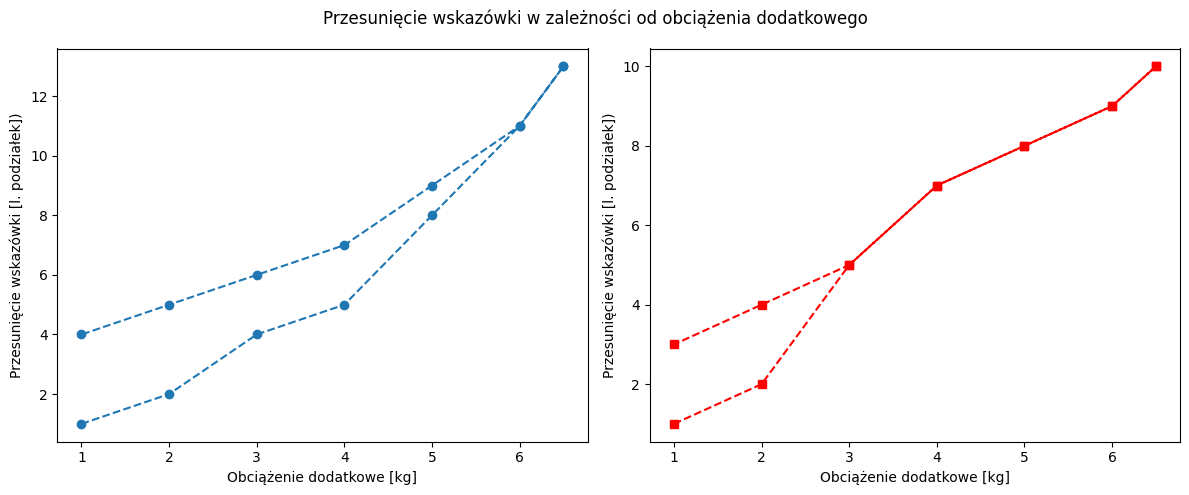
\includegraphics[width=1\linewidth]{histereza.png}
    \caption{Wydłużenie drutu po połączeniu następujących po sobie pomiarów prostymi (Źródło: opracowanie własne).}
    \label{fig:histereza}
\end{figure}

\section{Wykresy}

\begin{figure}[H]
    \centering
    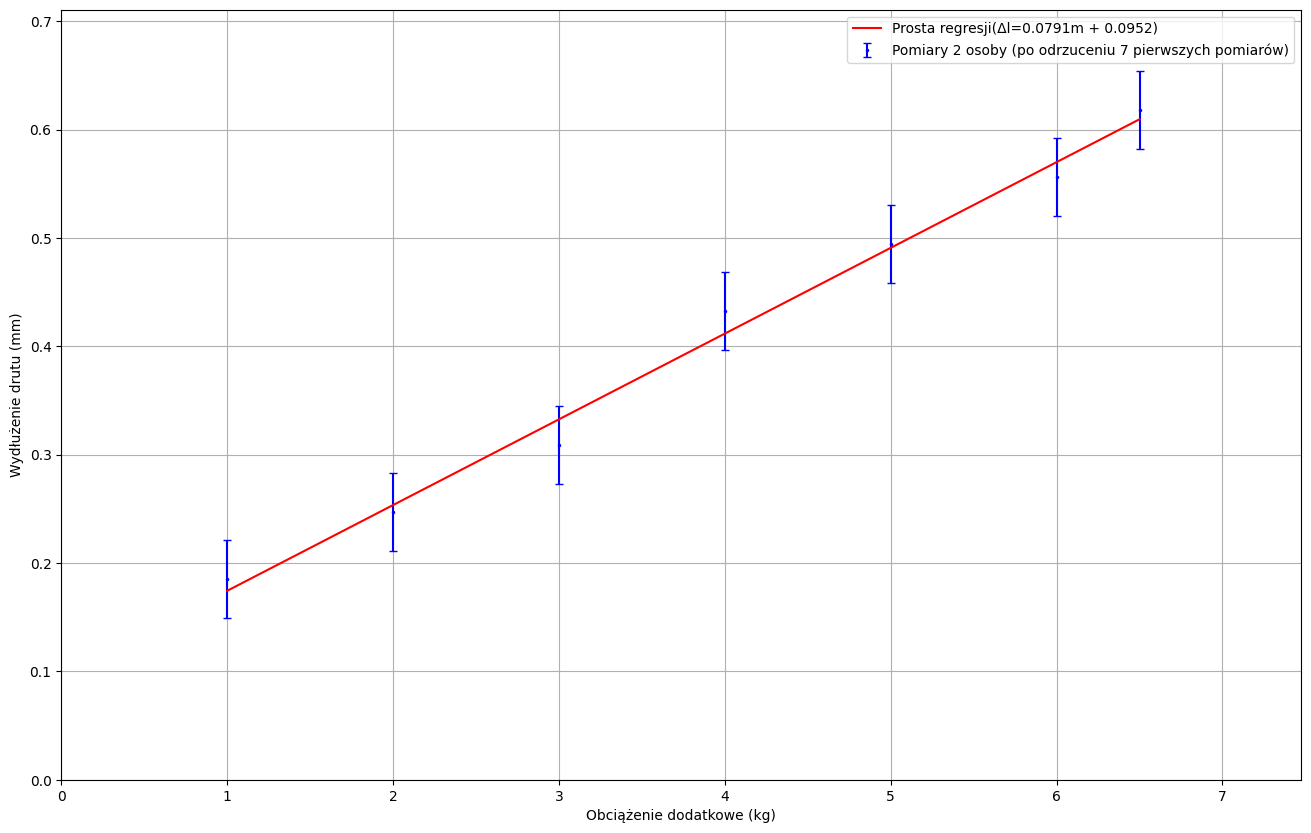
\includegraphics[width=1.2\linewidth,angle=90]{prosta_regresji.png}
    \caption{Nieodrzucone pomiary z nałożoną prostą regresji (Źródło: opracowanie własne)}
    \label{fig:prosta_regresji}
\end{figure}


\newpage

\begin{figure}[H]
    \centering
    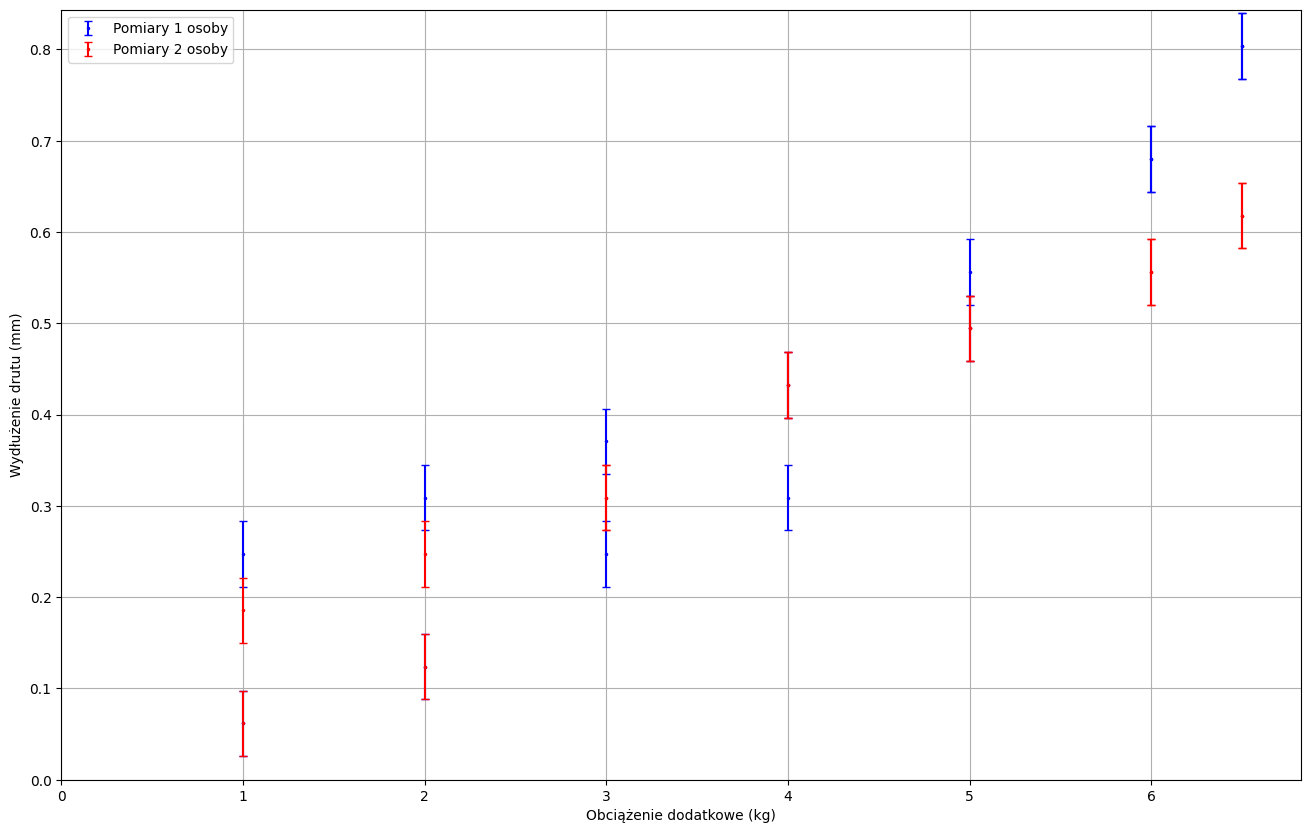
\includegraphics[width=1.2\linewidth,angle=90]{wszystkie_pomiary.png}
    \caption{Wszystkie pomiary z niepewnościami (źródło: opracowanie własne).}
    \label{fig:wszystkie_pomiary}
\end{figure}
\bibliographystyle{plain}
\bibliography{bibliography}

\end{document}
